\section{Equipment}
\subsection{Button Triggers}
To accurately observe the approximately-linear motion of a piano key, we feel a linear push-button switch is our best choice. We do not want any sort of locking mechanism because the key should be registered as ‘on’ when pressed and ‘off’ when released and each key will need two switches, which is a total of sixty-two total switches in the keyboard keys alone. Linear push-button switches provide this linear on-off response and come with a low price tag.

Since we want our project to feel as close to a professional MIDI controller as possible, we do not want our user to know there is a button being actuated separately from the key. This means our buttons should be almost silent and not provide any tactical feedback. To achieve these parameters we did our research and brought three types of buttons to debate: the \textit{Odseven Soft Tactile Button}, the \textit{Panasonic ESE-20d443}, and the \textit{Nidec Copal TR1-01}. The three choices offered are a single-pole single-throw linear push-button with a silicon cover. Their images and data are shown in \textit{Figure \ref{fig:buttons_fig}} and \textit{Table \ref{Tab:buttons_data}} .

\begin{figure}[h!]
  \centering
  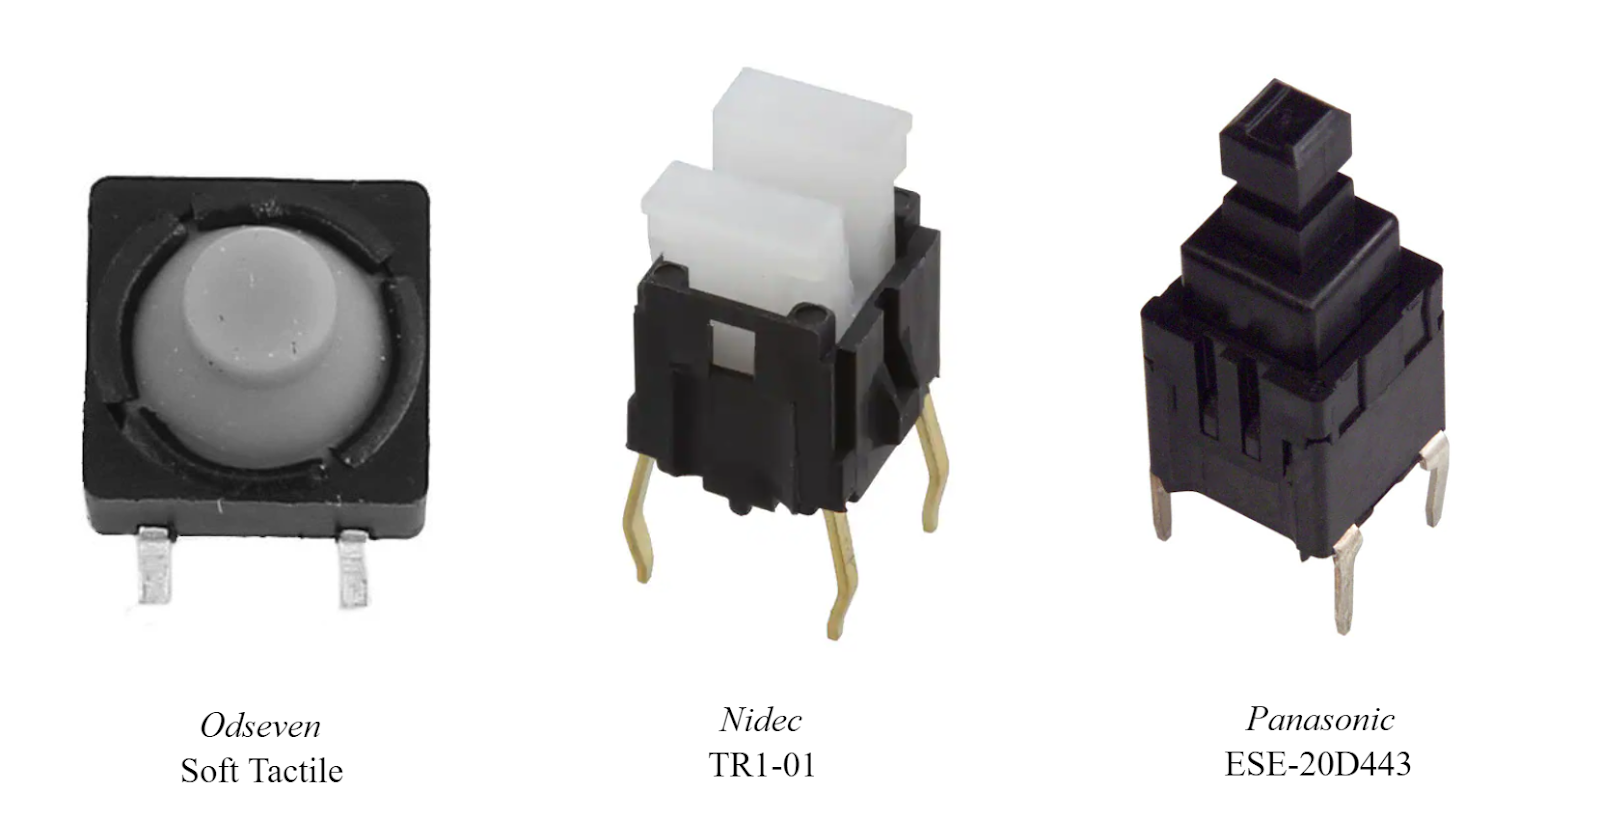
\includegraphics[width=\linewidth]{image/Buttons.png}
  \caption{A comparison of button options.}
  \label{fig:buttons_fig}
\end{figure}

\begin{table}[h!]
  \centering
  \resizebox{\textwidth}{!}{%
    \begin{tabular}{|l|l|l|l|}
      \hline
      Brand                           & Cost   & Quantity & Form Factor               \\ \hline
      Odseven                         & \$1.17 & 10       & 7.8mm x 7.8mm x 4.9mm     \\ \hline
      Nidec Copal Electronics         & \$0.54 & 1        & 5.9 mm x 7 mm x 9 mm      \\ \hline
      Panasonic Electronic Components & \$1.31 & 1        & 7.9 mm x 7.8 mm x 17.5 mm \\ \hline
    \end{tabular}}
  \caption{A comparison of costs for our button options}
  \label{Tab:buttons_data}
\end{table}

After debating which option would be the best for this project, we ultimately settled on the \textit{Odseven Soft Tactile} button for a few reasons. First, as we can see in \textit{Figure \ref{fig:buttons_fig}} and the accompanying \textit{Table \ref{Tab:buttons_data}} , The \textit{Nidec} and the \textit{Panasonic} buttons extend at least twice as high as the \textit{Odseven}. Although the taller buttons could provide more constant contact with the key and reduce the feeling of multiple actuations, the button would need to be in constant contact during the entire actuation of the key to make a difference in feel. On top of that, to receive information for velocity, we would need to place the buttons in different locations on the key and have different actuation distances from the key for each button. No matter our choice, constant contact would require two different types of buttons. Plus, the total actuation of the key is ten degrees for the white keys, fifteen degrees for the black keys, and we would need to find two buttons with extremely precise height and actuating distance.

The next reason we chose the \textit{Odseven Soft Tactile} button was because of the shape of the button itself. With a circular head and smallest actuation distance, it appears to be more versatile for our multistage actuation set-up, where the key is pressed before it presses the button itself. We could use a variety of rod shapes connected to the key and still get the \textit{Odseven} button to actuate properly. This will come in handy during the prototyping and reiteration of the project. It is also versatile enough to be used in other applications of the project, which will be discussed in their personal sections, and because the \textit{Odseven Soft Tactile} button comes in a pack of ten, this adds confidence that we will make the most use of each cent we spend. Additionally, the datasheets provided with all three of these devices do not offer a decibel reading of the button response. The only button which discussed sound was the \textit{Odseven} which claims to be “silent”. From our experience as musicians, we would much rather take a key that has an odd feeling when pressed over a key that clicks when pressed.

The final reason we chose the \textit{Odseven} button is the price. We have a budget goal of below five-hundred dollars and \textit{Odseven} sells this button, as well as \textit{Adafruit}, at a significantly lower price per button than the other options. Our project will be using sixty-four buttons in the keys alone and every unnecessary dollar spent on buttons will add up quickly.

\subsection{Springs}
By utilizing the measurement function of Solidworks we know that the minimum distance the spring will connect is 34.02 mm, shown in \textit{Figure \ref{fig:dimensions1}} and the maximum distance is 38.94 mm shown in \textit{Figure \ref{fig:dimensions2}}.

\begin{figure}[h!]
  \centering
  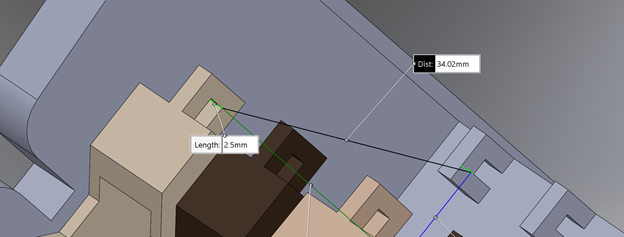
\includegraphics[width=\linewidth]{image/Dimensions1.png}
  \caption{A close-up on our keys' manufacturing specifications}
  \label{fig:dimensions1}
\end{figure}

\begin{figure}[h!]
  \centering
  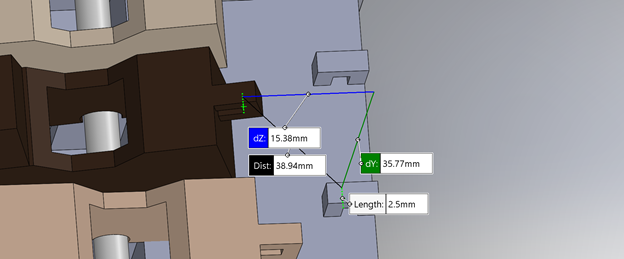
\includegraphics[width=\linewidth]{image/Dimensions2.png}
  \caption{A close-up on our keys' manufacturing specifications}
  \label{fig:dimensions2}
\end{figure}

From our knowledge of basic kinematics, we know that the force of a spring can be approximated by the equation:

\begin{equation} \label{spring_force}
  F = -k * x
\end{equation}

Where $ F $ is the force in Newton-meters, $ k $ is the spring constant determined by the manufacturing design and material of the spring, and $ x $ is the linear distance from the resting point (or state of equilibrium) of the spring. It is important in our design that the spring remains in tension while the key is at a zero degree actuation all the way to the 15 degree (or 10 degree for the natural keys) actuation. The reason this is important is to create a more even feel to the normal force while actuating the key. For example, if the $ x $ distance from equilibrium is the zero degree, or resting position, of the key, the force on the key would be zero when the key is not being used. Any amount of change in the position would create infinitely more force than its resting position. As Newton’s Third Law states, “for every action (force) in nature there is an equal and opposite reaction”, meaning that in our circumstance, the full actuation of the key will produce infinitely more force than its resting position as felt by the spring and the user pressing the key. Our aim is to allow the actuation of the key to feel as uniform as possible and since the force relationship with the spring’s distance is approximately linear, the percentage change per equal distance actuated is inversely proportional to the starting position of the key, $ x_{intial} $ . To gather a better understanding, this is a more realistic example.

Obviously if the spring is starting at rest any distance traveled from rest would create infinitely more force than when it is at rest. Now, using the keys as a perfect example, let’s say the max actuation distance is a fixed value. In our case, the maximum actuation for any of our keys is 4.92 mm. For example purposes, let’s say the constant value $ k $ is equal to one. If this key is starting at an initial $ x $ value of 1 mm and traveling to 5.92 mm (the maximum actuation distance plus the initial position), the initial force would be 1m Nm and the final force would be 5.92 m Nm. This is a 492\% change in force over the course of the actuation. If the key starts the spring at $ x $ equals 10 mm and finishes at 14.92 mm, the starting force would be 10 m Nm and the final force would be 14.92 m Nm, creating a 49.2\% change in force over the actuation of the key. We can see how the starting position of the spring affects the overall force change over distance in \textit{Table \ref{Tab:x_force}}.

\begin{table}[h!]
  \centering
  \resizebox{\textwidth}{!}{%
    \begin{tabular}{|l|l|l|l|l|l|l|}
      \hline
      X initial (mm) & Constant K & Max Actuation (mm) & X Final (mm) & Force Initial (m N*m) & Force Final (N*m) & Force \% Change \\ \hline
      5              & 2          & 4.92               & 9.92         & 10                    & 19.84             & 98.4            \\ \hline
      10             & 2          & 4.92               & 14.92        & 20                    & 29.84             & 49.2            \\ \hline
      20             & 2          & 4.92               & 24.92        & 40                    & 49.84             & 24.6            \\ \hline
      30             & 2          & 4.92               & 34.92        & 60                    & 69.84             & 16.4            \\ \hline
      50             & 2          & 4.92               & 54.92        & 100                   & 109.84            & 9.84            \\ \hline
      100            & 2          & 4.92               & 104.92       & 200                   & 209.84            & 4.92            \\ \hline
    \end{tabular}}
  \caption{The tabularized relationship between stretch and tension in a spring}
  \label{Tab:x_force}
\end{table}

From the table it is obvious that, with a fixed maximum actuation, the percent change in force per $ x $ distance is inversely proportional to the initial $ x $ location.

Although this information is valuable and shows the important aspect that we should be wary of the force percent change over distance, it is also important to take into consideration the strength of the material as well. In an ideal world, aiming for a zero percent change in force over distance would mean starting the initial $ x $ value at an infinite distance from its equilibrium. This is obviously not possible as the spring would break long before an infinite distance. We do not have to worry about starting at an infinite distance and we also recognize that the plastic holding the spring will break long before a metal spring breaks, but we do need to take into account the possibility of the spring deforming by being stretched too long. Therefore, creating the best initial distance to reduce the percent change of force over distance is a balance act with the material properties of the spring itself.

Since we do not have any members with mechanical engineering experience on our team, we are more or less, attempting to do this by trial and error. Obviously we are utilizing common sense to make our decisions, but we find it difficult to justify all of our choices through complete objective reasoning. We decided to debate between six different types of springs under the following pretenses. First, the resting position should be less than the zero degree actuation distance of the key. Second, the starting force of the spring should be approximately one pound per square inch. Third, the maximum distance of the spring should not be below the maximum actuation distance necessary. By utilizing trusted websites our group decided on debating the springs shown in \textit{Table \ref{Tab:spring_brand}}.

\begin{table}[h!]
  \centering
  \resizebox{\textwidth}{!}{%
    \begin{tabular}{|l|l|l|l|l|l|l|}
      \hline
      Brand         & Cost    & Quantity & Initial Length & Max Length & Pounds per Distance & Starting Load \\ \hline
      McMaster-Carr & \$13.80 & 2        & 30.2 mm        & 58.1 mm    & .241 lbs/mm         & 1.08 lbs      \\ \hline
      McMaster-Carr & \$12.35 & 2        & 30.6 mm        & 49.2 mm    & .319 lbs/mm         & 1.49 lbs      \\ \hline
      McMaster-Carr & \$10.90 & 2        & 31 mm          & 53.6 mm    & .13 lbs/mm          & .7 lbs        \\ \hline
      WB Jones      & \$3.08  & 1        & .875 inch      & N/A        & .8 lbs/in           & .15 lbs       \\ \hline
      WB Jones      & \$3.08  & 1        & 1 inch         & N/A        & 0.67 lbs/in         & 0.15 lbs      \\ \hline
      WB Jones      & \$2.33  & 1        & 1 inch         & N/A        & 1.38 lbs/in         & .26 lbs       \\ \hline
    \end{tabular}}
  \caption{A comparison of costs for our spring options}
  \label{Tab:spring_brand}
\end{table}

Although the WB Jones offers cheaper options, it is more difficult to distinguish which spring would be appropriate as they do not provide a maximum length nor any type of image to distinguish the proportions of the springs. Before coming across any of these options, we made sure each selection was a corrosion resistant tension spring equipped with a hooked end to easily be incorporated to our project. Due to the lack of concrete imagery for the references we ultimately decided to focus on the McMaster-Carr options. Images of those options are as follows: the 30.2 mm spring, the 30.6 mm spring, and the 31 mm spring in \textit{Figure \ref{fig:springs}} each provided by McMaster-Carr.

Since we are unaware of the mechanical properties associated with the diameter of the spring wire, the actual feel in the implementation of the pounds per inch or millimeter, or the utilization of a spring in this mechanical system, we are going to decide by approximate parameters and look of each spring. To play it safe, we are choosing to initially purchase the spring which has the least amount of lbs/m. There is no reliable documentation on exactly how much force it takes to compress a piano key and therefore we will be attempting trial and error during the second semester of this project to find the best spring load.

After evaluating the cost and difference of each type of spring, we ended up using a 2.5 in x .25 in x .035 in zinc plated extension springs to create the actuation. These were purchased from Ace Hardware and cost significantly less than any of the previous options.

\newpage
\begin{figure}[h!]
  \centering
  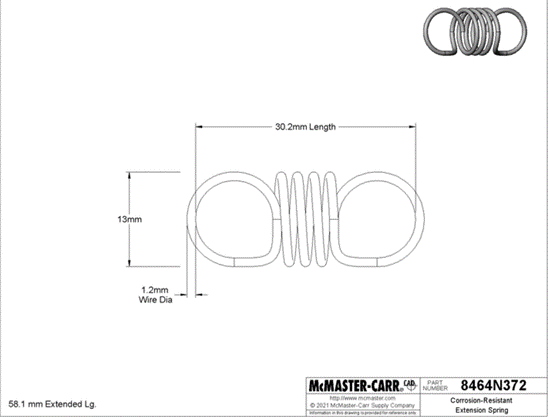
\includegraphics[width=0.6\linewidth]{image/Spring1.png}
  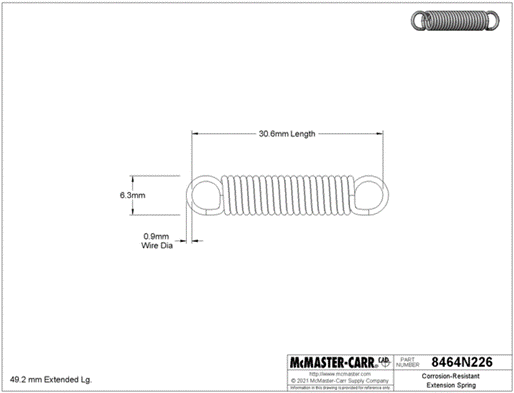
\includegraphics[width=0.6\linewidth]{image/Spring2.png}
  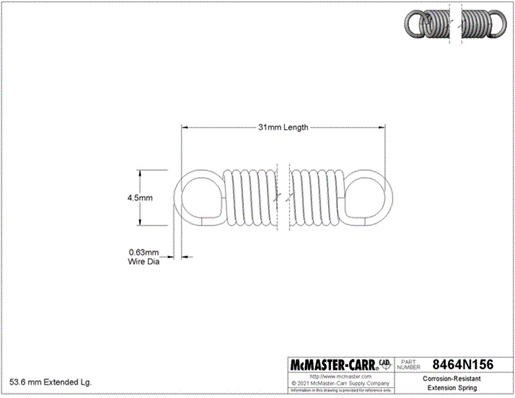
\includegraphics[width=0.6\linewidth]{image/Spring3.png}
  \caption{A comparison of our spring options}
  \label{fig:springs}
\end{figure}
\newpage

\subsection{Key Rail}

As discussed in the \textbf{Prototyping} subsection of \textbf{Implementation}, we are no longer attempting to 3D print the rail itself. To replace this 3D printed rail, we bought three alternatives to discuss and debate shown in \textit{Table \ref{Tab:rail_brand}}.

\begin{table}[]
  \centering
  \begin{tabular}{|l|l|l|l|l|}
    \hline
    Brand  & Cost    & Quantity & Form Factor  & Material        \\ \hline
    Amazon & \$11.89 & pack     & 1/8 inch     & 'Natural Wood'  \\ \hline
    Amazon & \$5.99  & 2        & 4mm x 300 mm & Stainless Steel \\ \hline
    K\&S   & \$7.14  & 3        & 4mm x 300 mm & Brass           \\ \hline
  \end{tabular}
  \caption{A comparison of material costs for key rail options}
  \label{Tab:rail_brand}
\end{table}

At the beginning of the discussion, we immediately eliminated the option of the ‘Natural Wood’ dowels. Our aim is to create a device that is not only functional, but also robust and can handle the perturbations that come along with a portable device. Wood cannot handle nearly as much force as metal and it is difficult to even compare that type of wood with the other options because there was little descriptive information on the type of wood other than ‘natural’.

When comparing the Stainless Steel rods to the Brass rods, this choice was difficult. They are both 4 mm x 300 mm which is wonderful for our application, they both ship from Amazon prime which means we would not have to worry about delivery time, they both are consistently in stock, and they are both close enough in price that it is negligible. To decide, we first took a look at the strength of each rod.

According to material-properties.org the yield strength of brass is about 95 MPa, where the yield strength of stainless steel is about 170 MPa. Next we discussed the properties of each metal over time. As brass continues to be used and exposed to the elements it begins to oxidize, or rust, quickly to a greenish-blue material. Stainless steel does not oxidize. Although this factor is not too difficult to address, it is important to recognize that a rusted material has a higher coefficient of friction over its non-rusted counterpart. If we want the keys to continue actuating over time with as little degradation in actuation ease, it is important that the rod which the key is actuating over does not increase in friction over time. It is worth noting that stainless steel does in fact wear down, but the lack of rust will keep the actuation in better condition than if the rod actuated. For these reasons, we felt it was best to choose the 4 mm x 300 mm stainless steel rod for our project.

\subsection{Display}

While debating on which screen to use, our group came up with two options, shown in \textit{Table \ref{Tab:display_brand}}.

\begin{table}[]
  \centering
  \begin{tabular}{|l|l|l|l|}
    \hline
    Brand   & Cost    & Quantity & Display Size \\ \hline
    Newsoul & \$84.99 & 1        & 7 inch       \\ \hline
    ElecLab & \$49.90 & 1        & 5 inch       \\ \hline
  \end{tabular}
  \caption{Comparison of display screen options}
  \label{Tab:display_brand}
\end{table}

We were torn between utilizing a physical button oriented user interface and a touch screen oriented interface. As a group, we decided that allowing our end-users the option of a touch screen is more up-to-date with current technology. Not only that, the members of our CS division for this project felt the design and creation of a touch based user interface would be easier to code on the backend and easier to operate on the user’s end. Because of this, we eliminated the choice of any non-touch screens for this project. Next, we discussed whether a capacitive or resistive touch screen would be more appropriate. A general rule of thumb for touch screens is: capacitive touch screens are often more expensive, but offer multi-point touch recognition. Resistive touchscreens are often cheaper, but only allow single-point navigation. We felt resistive touch screens are outdated and decided that adding the extra cost of a capacitive touchscreen for the design would be worth the ease of use and a more professional feel to the finalized product.

We also wanted to make sure there was enough room on the screen for the user to easily view the software user interface and be able to navigate the software. Sadly, none of the options offered by the group had a datasheet reliable enough to find the power usage of the screen. Luckily, each screen is designed to be operated by a Raspberry Pi and claims to work well with the device, therefore we can be assured that the current usage is within the limits a Raspberry Pi can offer. This is later discussed in the Batteries section of this paper. Ultimately, we decided to choose the seven-inch display to offer the greatest experience for our end users that fits within our budget.

\subsection{Octave Up/Down}

With almost every electric keyboard there is a trigger on the device for Octave Up and Octave Down. These buttons simply take the input for each key and represent it as the corresponding note in either the octave above that key or the octave below that key. For example, when octave up is triggered, a key that is usually represented as a C in the 1st octave would be sent to the device as a C in the 2nd octave. Octave down shifts the key in the other direction such that a key in the 1st octave would be sent to the device as a key in the 0th octave. It is important to note that there are about 11 octaves in the audible hearing range from C-1 with a frequency around 8 Hz to B10 with a frequency around 31 kHz. The pitch names, MIDI corresponding values, and frequencies can be seen in \textit{Table \ref{Tab:note_frequency}}. Due to the range of octaves and the fact that our keyboard will only have two and half octaves present, it is to be expected that the octave up and octave down buttons should have the option to be pressed multiple times and add additional octave shifts in the specified direction.

\begin{table}[]
  \centering
  \resizebox{\textwidth}{!}{%
    \begin{tabular}{l}
      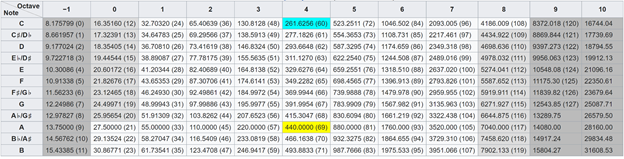
\includegraphics{image/NoteFrequency}
    \end{tabular}}
  \caption{The tabularized relationship between MIDI values and their tonal frequency}
  \label{Tab:note_frequency}
\end{table}

In between the Octave Up and Octave Down buttons we will have a single button to play and pause the MIDI notes already inputted into the DAW. This will operate by simply triggering the opposite of which action the playback is currently performing. When paused this button will play the MIDI data, while playing this button will pause the playback of the MIDI roll.

Below the Play / Pause button will be a Record button. This is used to input MIDI data in real time. After the button is first triggered, it will record all inputs from the keyboard from there after. After the user has recorded what they want, they can press the record button again and the recording will stop and save all MIDI data from the time between the first and second button press.

\subsection{Volume Control}

Almost immediately upon the start of our discussion, we decided that a sliding potentiometer would be best for volume control. Not only is it easy to hook up to any device, like any potentiometer, but it also allows physical and visual feedback of the volume. We plan to use an analog general input output pin (GPIO) directly tied from the potentiometer into the Raspberry Pi. After reading the value of the potentiometer, this will be translated to the volume we expect to produce.

\begin{figure}[h!]
  \centering
  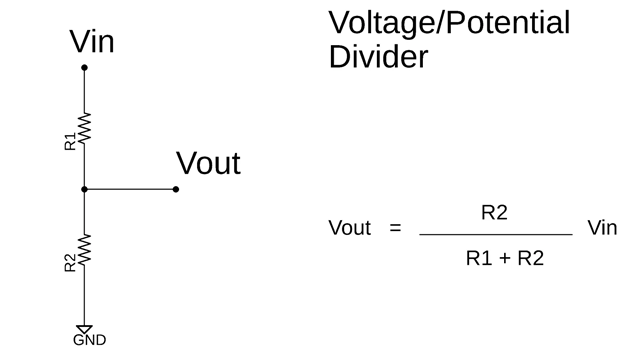
\includegraphics[width=\linewidth]{image/VoltageDiv.png}
  \caption{The voltage divider}
  \label{fig:voltage_div}
\end{figure}

A potentiometer works by using the concept of a voltage divider which is shown in \textit{Figure \ref{fig:voltage_div}} from electronicclinic.com. There is a $ V_{in} $ supplied by a source, in our case the Raspberry Pi, which is connected to a variable resistor. That variable resistor is connected to the actuating lever which is seen on the outside of the potentiometer. As the lever slides upwards along the potentiometer, the resistance increases and creates a change in the output voltage, which is connected to the actuating lever as well. By knowing the input voltage and reading the output voltage, the device is able to tell from the equation given in \textit{Figure \ref{fig:voltage_div}} where on the slider the lever is located. By using this value, we will translate that the bottom position of the potentiometer is zero output volume and the top position of the sliding potentiometer is full or 100\% volume.

Most musicians who have worked in the synthetic side of music composition or performance have worked with sliding potentiometers in this manner and therefore gives another reason why we, as a team, were drawn to the idea of using a sliding potentiometer over a rotating potentiometer. We easily could have chosen to use a rotating potentiometer, but these are more often used in amplifiers, guitars, and other types of instruments that are not the keyboard. At the end of the day, it all comes down to user preference and our team prefers this decision. We also chose to gather the pack of ten over a single sliding potentiometer because it was not only an easier option over Amazon, but it also provides the components in case we would like to add analog synthetic effects to our device.

The device we chose is the WMCONGCONG 10 kOhm sliding potentiometer. This device provides 1023 data points over the course of its actuation which is more than enough to reduce these data points into volume markers. We chose this device because of the cheap cost of \$14.99 for ten units and the small form factor. It was imperative that the sliding potentiometer fit within the vertical limit of the UI cover for the device. As can be seen in the Keyboard Design section of the document, the slot to the right of the screen which is designed to house this potentiometer is well within our limits and fits aesthetically as well.

We do recognize that the actuating lever for this device is a bit homely, but we were able to design and print a cap for the lever and create a more authentic sliding volume potentiometer feel that many mixers and synthetic instruments use.

\begin{figure}[h!]
  \centering
  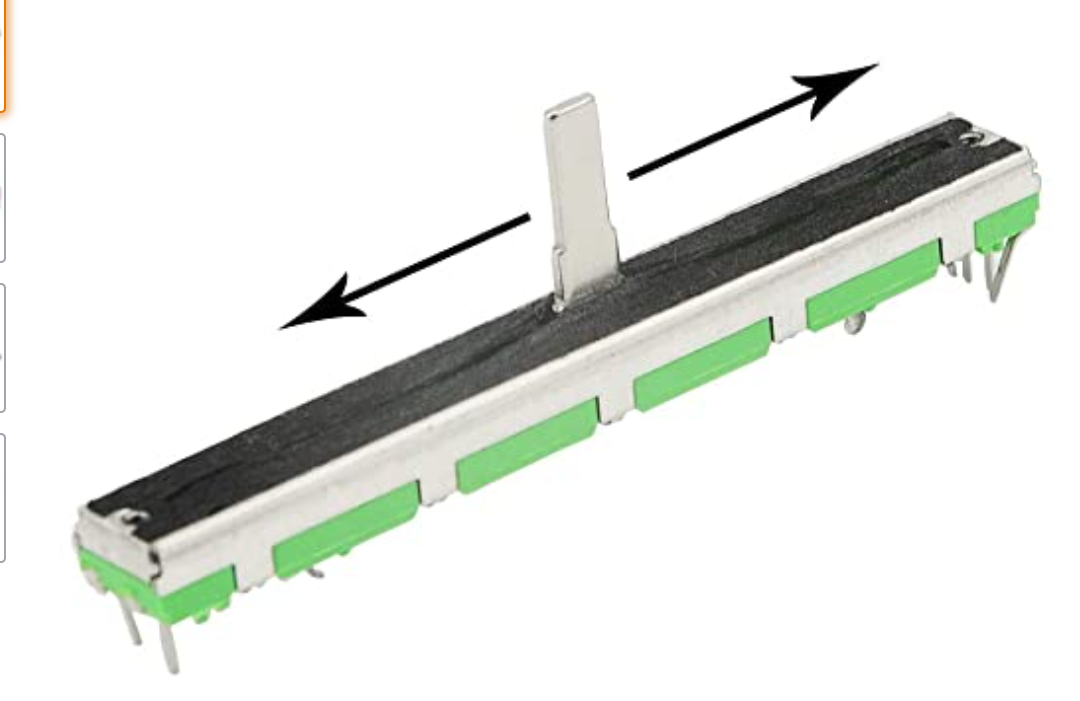
\includegraphics[width=0.5\linewidth]{image/Potentiometer.png}
  \caption{WMCONGCONG 10 kOhm sliding potentiometer}
  \label{fig:potentiometer}
\end{figure}


\subsection{Audio Jack}

The audio jack, also known as the headphone jack or auxiliary jack, is the location where the user can input their headphones to listen to the audio being produced by the Raspberry Pi. There are two major types of audio jacks: mono and stereo. Mono headphone jacks are audio outputs that can only send one audio signal out. This means, if an individual is using headphones, the audio in the right ear will be the exact same audio produced in the left ear. Stereo is the counterpart to mono, and can channel two or more audio signals from a single jack. This means, if all is set up correctly, that the left and right speakers can produce two different signals and create a fuller environment for the listener. This can be further understood in the mechanical drawing shown in \textit{Figure \ref{fig:mono}} and \textit{Figure \ref{fig:stereo}} which are the mono and stereo female drawings respectively.

\begin{figure}[h!]
  \centering
  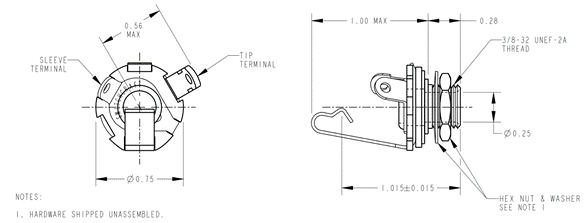
\includegraphics[width=\linewidth]{image/Mono.png}
  \caption{The mono jack option}
  \label{fig:mono}
\end{figure}
\begin{figure}[h!]
  \centering
  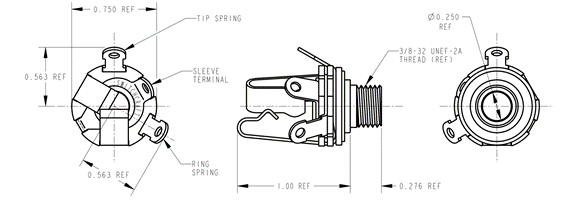
\includegraphics[width=\linewidth]{image/Stereo.png}
  \caption{The stereo jack option}
  \label{fig:stereo}
\end{figure}

As you can see from \textit{Figure \ref{fig:mono}} and \textit{Figure \ref{fig:stereo}}, each jack is designed with two different pinouts. The mono headphone jack has only a tip and sleeve pin while the stereo jack has a tip, sleeve, and ring pin to connect to the Raspberry Pi,  each connecting to the corresponding location on the male input jack.

Considering our user interface is more about producing a new type of melody designed by artificial intelligence and machine learning and less about the production value itself, we believe it is best to go with the mono headphone jack. Not only is it cheaper, as seen in \textit{Table \ref{Tab:jack_brand}}, but it is also easier to code, connect, work with, and troubleshoot.

\begin{table}[]
  \centering
  \begin{tabular}{|l|l|l|l|l|}
    \hline
    Brand       & Cost   & Quantity & Form Factor         & Notes  \\ \hline
    Switchcraft & \$2.15 & 1        & 10 mm mounting hole & Mono   \\ \hline
    Switchcraft & \$2.25 & 1        & 10 mm mounting hole & Stereo \\ \hline
  \end{tabular}
  \caption{A comparison of costs for our audio jack options}
  \label{Tab:jack_brand}
\end{table}

\subsection{T-Cobbler}

One big misfortune about the Raspberry Pi compared to Arduino is that the Raspberry Pi model we chose is not as easily accessible to hardware prototyping as any of the Arduino boards. On the flip side, we still want to be able to connect many different analog devices such as the octave up and octave down buttons as well as the headphone jacks and hopefully speakers by the end of the project. To combat this, our group decided it would be in our best interest to purchase a Pi T-Cobbler Plus -- GPIO breakout board for prototyping. This device costs less than ten dollars and will allow for easier prototyping by connecting the GPIO pins on the Pi to a breadboard, shown in \textit{Figure \ref{fig:tcobbler}}.

\begin{figure}[h!]
  \centering
  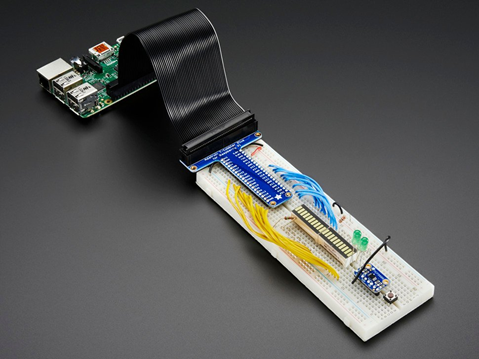
\includegraphics[width=\linewidth]{image/TCobbler.png}
  \caption{A sample of our T-Cobbler usage in prototyping}
  \label{fig:tcobbler}
\end{figure}
\newpage

After prototyping, we simply used the pinout on the Pi to connect the devices.

\subsection{MIDI Translation}
Before recording or playing the note on the Raspberry Pi, we need a device that will be able to interpret the analog signals from the keyboard and translate the keystrokes into MIDI data. After the data is acquired it will be sent via USB to the Pi as a MIDI input, but which device should we use? After a short discussion, our group felt that Arduino or one of the many arduino clones would be our best choice due to its ease of integration and the familiarity our members have working in C code. With the integrated multiplexers in the PCB our MCU (Microcontroller Unit) only needed six digital I/O pins for data, one input for voltage in, and one input for group. The cheapest board models that met this description are the Arduino Nano, Arduino Micro, and Arduino Nano-Every. Here is a quick comparison chart of the following devices with the specs we took into account.

\begin{table}[]
\centering
\begin{tabular}{|l|l|l|l|}
\hline
Device            & Arduino Nano & Arduino Micro & Arduino Nano-Every \\ \hline
Digital I/O       & 22           & 20            & 12                 \\ \hline
USB data transfer & Yes          & Yes           & Yes                \\ \hline
Cost              & \$20.70      & \$18.40       & \$11.90            \\ \hline
\end{tabular}
\end{table}

Ultimately, every board available on the Arduino website has the specifications we need to be able to execute the project. Our choice ended up coming down to cost and keeping the project within budget as best as possible. Even with the cheapest option, we were able to have enough digital I/O pins with an included 8 analog pins.

\begin{figure}[h!]
  \centering
  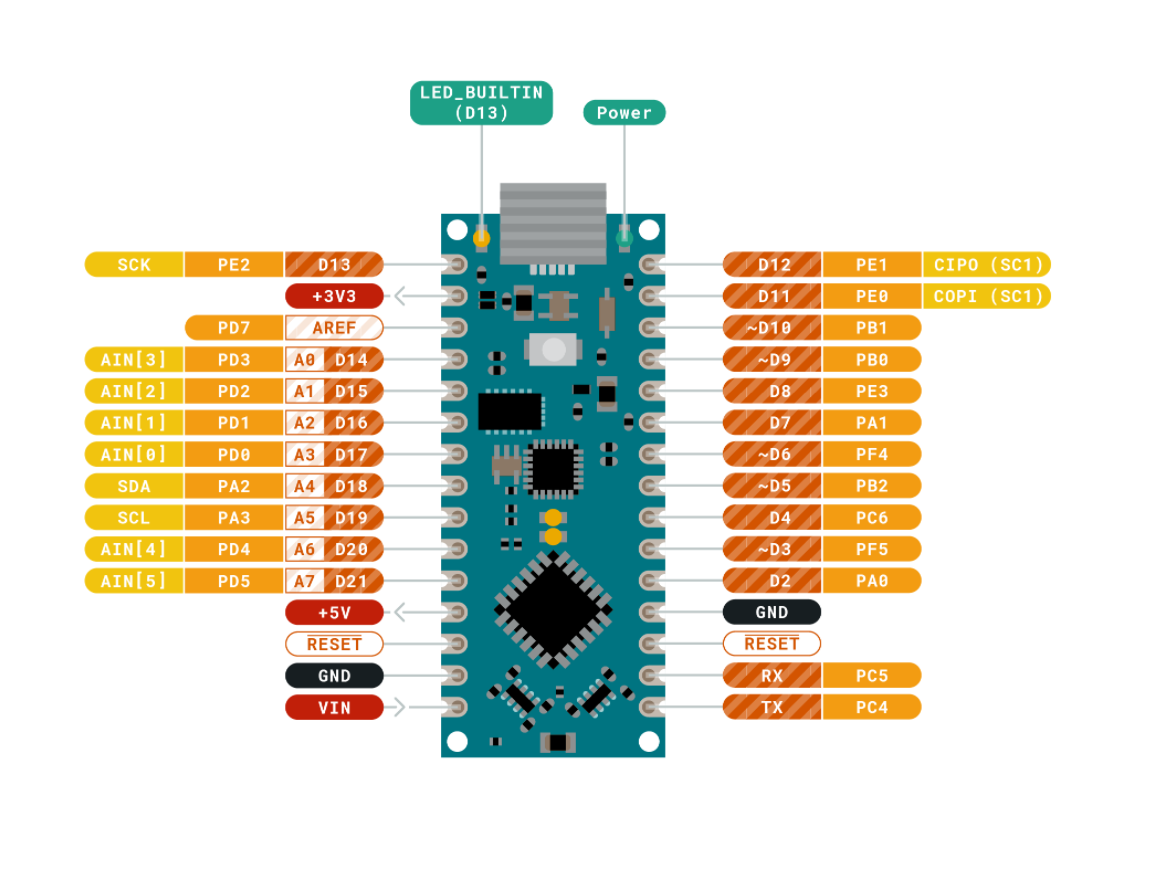
\includegraphics[width=0.8\linewidth]{image/Pins.png}
  \caption{The set of analog pins available through our Arduino}
  \label{fig:pins}
\end{figure}

Luckily for us it was necessary to utilize those analog pins for the volume slider since the Raspberry Pi does not have an ADC (analog to digital converter). We also chose this device because it had the smallest form factor of the three. Although each device is relatively small and the size itself would not have impacted the project greatly, we figured every little but counts in a fully portable device.

\subsection{Batteries}

Due to the limited options of batteries that we could reasonably have in our possession during the manufacturing process, one of our CS members felt our best choice was purchasing our device battery from a vape shop. TBy doing this we were able to ensure our device would be in our possession on time, but sadly reduced our variety of options. This endeavor was supported by the rest of the group because vape batteries are used to power heating devices: one of the greater current and watt demanding devices we know of. From the measurements we have of the charging device we purchased, our best option in store were 18650 batteries. These are 2.6 amp hour batteries. 2.6 amp hours is right on the cusp of being able to maintain our 2.5 amp device for about an hour. We used two of these batteries and therefore deduced that we should be able to power our device for around 2 hours on a single charge. This is quite short for a portable device, but it was the best option we were able to possess in our time and charging constraints. These batteries are shown in the figure below.

\begin{figure}[h!]
  \centering
  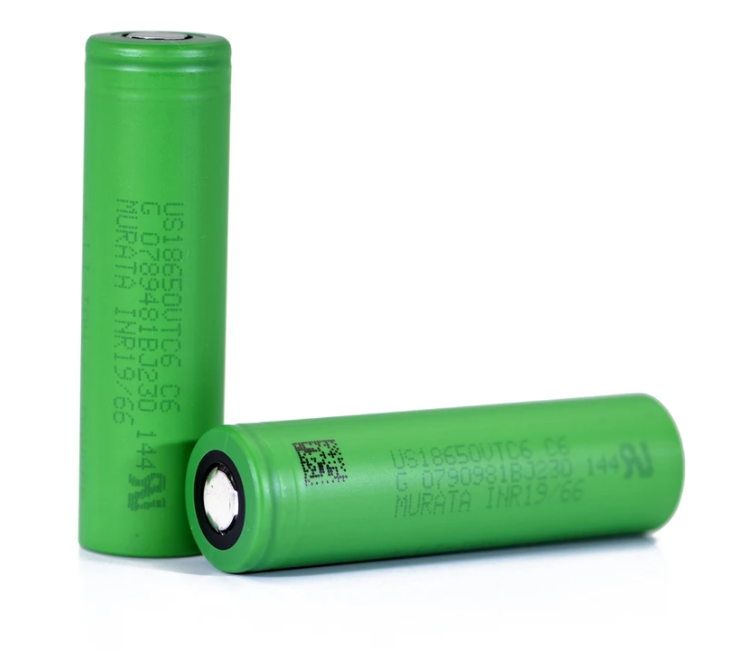
\includegraphics[width=0.8\linewidth]{image/Batteries.png}
  \caption{The batteries used to power our device}
  \label{fig:batteries}
\end{figure}

\subsection{Printer Filament}

Since we are using an at-home 3D printer, our choices were limited. None of the members in our group felt comfortable changing the specifications of the device and therefore were limited to the settings already established in the printer. Our choices from the very beginning were Sunlu’s PLA and PLA+ options. Considering the entire model was going to be created with this plastic, we did not want to go with the weaker option. The major difference between PLA and PLA+ is that the PLA+ is advertised as a more durable, more reliable printing plastic. Due to this reason, we bought 3 kgs of PLA+ filament: 2 kgs of black filament and 1 kg of white filament to model a keyboard as accurately as possible.
